\documentclass[11pt]{article}

% load some asm stuff -
\usepackage{amssymb}
\usepackage{amsmath}
\usepackage{amsthm}
%\usepackage{palatino,lettrine}
\usepackage{fancyhdr}
\usepackage{epsfig}
\usepackage[square,sort,comma,numbers]{natbib}
\usepackage{simplemargins}
\usepackage{setspace}
\usepackage{wrapfig}
\usepackage{hyperref}
%\usepackage{boiboites}
\usepackage[margin=0pt,font=small,labelfont=bf]{caption}
\newcommand{\boldindex}[1]{\textbf{\hyperpage{#1}}}
\usepackage{makeidx}\makeindex
\bibliographystyle{plos2015}

\usepackage{algpseudocode}
\usepackage{algorithm}


% Set the size
%\textwidth = 6.75 in
%\textheight = 9.75 in
%\oddsidemargin = 0.0 in
%\evensidemargin = 0.0 in
%\topmargin = 0.01 in
%\headheight = 0.0 in
%\headsep = 0.25 in
%\parskip = 0.15in
% \doublespace
\setallmargins{1in}

\newtheorem{example}{Example}[section]
\newtheorem{thm}{Theorem}[section]
\newtheorem{property}{Property}[section]

\theoremstyle{definition}
\newtheorem{defn}[thm]{Definition}

\makeatletter
% \renewcommand\subsection{\@startsection
% 	{subsection}{2}{0mm}
% 	{-0.05in}
% 	{0.05\baselineskip}
% 	{\normalfont\normalsize\bfseries}}
\renewcommand\subsubsection{\@startsection
	{subsubsection}{2}{0mm}
	{-0.05in}
	{-0.5\baselineskip}
	{\normalfont\normalsize\itshape\bfseries}}
\renewcommand\paragraph{\@startsection
	{paragraph}{2}{0mm}
	{-0.05in}
	{-0.5\baselineskip}
	{\normalfont\normalsize\itshape}}
\makeatother
\linespread{1.1}

\fancypagestyle{proposal}{\fancyhf{}%
	\fancyhead[RO,LE]{\thepage}%
	\fancyhead[LO,RE]{CHEME 5660 Derivatives and Derivative Pricing}%
	\renewcommand\headrulewidth{1pt}}
\pagestyle{proposal}

\usepackage{mdframed}
\definecolor{lgray}{rgb}{0.92,0.92,0.92}
\definecolor{antiquewhite}{rgb}{0.98,0.92,0.84}
\definecolor{lightskyblue}{rgb}{0.93,0.95,0.99}

% defn environment
\mdfdefinestyle{theoremstyle}{% 
    linecolor=black,linewidth=1pt,% 
    frametitlerule=true,% 
    frametitlebackgroundcolor=lgray, 
    innertopmargin=\topskip,} 
\mdtheorem[style=theoremstyle]{definition}{Definition}

% concept environment
\mdfdefinestyle{conceptstyle}{% 
    linecolor=black,linewidth=1pt,% 
    frametitlerule=true,% 
    frametitlebackgroundcolor=lightskyblue, 
    innertopmargin=\topskip,} 
\mdtheorem[style=conceptstyle]{concept}{Concept}
\newcommand{\newterm}[1]{{\it #1}}

% Single space'd bib -
\setlength\bibsep{0pt}

\renewcommand{\rmdefault}{phv}\renewcommand{\sfdefault}{phv}
%\newboxedtheorem[boxcolor=black, background=gray!5,titlebackground=orange!20,titleboxcolor = black]{color_box_example}{Example}{test}

% Change the number format in the ref list -
\renewcommand{\bibnumfmt}[1]{#1.}

% Change Figure to Fig.
\renewcommand{\figurename}{Fig.}
\usepackage{enumitem}
\setlist{noitemsep} % or \setlist{noitemsep} to leave space around whole list

%Joycelyn Chan, Joshua Lequieu, Michael Paull, Chidanand Balaji, Ryan Tasseff
%Our derivation follows closely the earlier development of Fredrickson \citep{Fredrickson:1976fk}.

% Begin ...
\begin{document}

%\begin{titlepage}
{\par\centering\textbf{\Large Unit 3: Introduction to Derivatives and Derivative Pricing}}\\
{\par \centering \large{CHEME 5660: Derivatives and Derivative Pricing}}
\vspace{0.2in}
{\par \centering \large{Jeffrey D. Varner}}
\vspace{0.05in}
{\par \centering \large{Smith School of Chemical and Biomolecular Engineering}}
{\par \centering \large{Cornell University, Ithaca NY 14853}}
% \vspace{0.1in}
% {\par \centering \small{Copyright \copyright\ Jeffrey Varner 2018. All Rights Reserved.}}\\

%\end{titlepage}
\date{}
\thispagestyle{empty}

\setcounter{page}{1}

\tableofcontents
\clearpage
\listoffigures
\clearpage
\listofalgorithms
\clearpage

\section{Introduction}
Derivatives are one of the three primary financial instrument categories: derivatives, equity (i.e., shares of stock), and debt (i.e., bonds and mortgages). 
Derivatives provide payoffs that depend on the value of other assets, such as commodities, bonds, stocks, or market indexes. 
Thus, the value of a derivative is based mainly on the price movements of an underlying asset, e.g., stocks, commodities, currencies, etc. 
This course will focus exclusively on options, a derivative product that uses stock as its underlying asset. 
Like bonds, options are contractural agreements between buyers and sellers to conduct a particular transaction at some later date. 
Options, derivatives that use equity, i.e., shares of a stock or an exchange-traded fund, as their underlying asset, 
are structured agreements between a buyer and a seller that give the option buyer the right, but not the obligation, 
to execute the transaction described in the contract, i.e., to buy (or sell) an underlying asset in some predetermined way in a specified time frame. 
The predetermined price is the strike price, and the specified period is the contract's lifetime, where the lifetime ends on the expiration date. 

Investors can use options and other derivatives to \href{https://www.investopedia.com/terms/h/hedge.asp}{hedge} against future asset price movements or for speculation. 
For example, a trader can buy an option contract instead of shares of an underlying stock to generate profits from the underlying stock's price movements, 
typically at a lower cost than the corresponding block of shares. Options contracts are traded on exchanges throughout the world; 
the \href{https://www.cboe.com}{The Chicago Board Options Exchange} is the largest options exchange in the United States, 
responsible for approximately 33\% of the daily options trading volume in the United States (about 32 million contracts are traded each day in the United States in 2023). 
Worldwide, in 2023, there were \href{https://www.fia.org/fia/articles/global-futures-and-options-volume-hits-record-137-billion-contracts-2023}{approximately 137 billion derivatives contracts traded annually}.
Options are also attractive because they offer \href{https://www.merrilledge.com/investment-products/options/options-trading-leverage-risk}{leverage}, 
i.e., an option contract can control a unit of asset, e.g., 100 shares of a stock, 
at a cost that is typically less than the market value of that asset. 
This allows option buyers to pay a relatively small premium for market exposure in relation to the value of the underlying asset. 
An option buyer can see significant gains from comparatively small percentage moves in the underlying asset's price. 
However, leverage also has a considerable downside. 
For example, if the underlying asset price does not rise or fall as anticipated during the lifetime of the option contract, 
leverage magnifies the investment's percentage loss.

In this module, we'll begin our study of derivatives, and options in particular, by focusing on European-style options contracts.
For European-style contracts, holders can only exercise their right on the expiration date.
However, for American-style contracts, which we'll consider later, the holder can exercise their right on or before the expiration date.
We'll study the two types of options contracts: \texttt{call} contracts and \texttt{put} contracts (Fig. \ref{fig:options-schematic}).

% The holder of the option pays a premium for the right to buy or sell the underlying asset. 
% The premium is the price of the option.

\begin{figure}[ht]
    \centering
    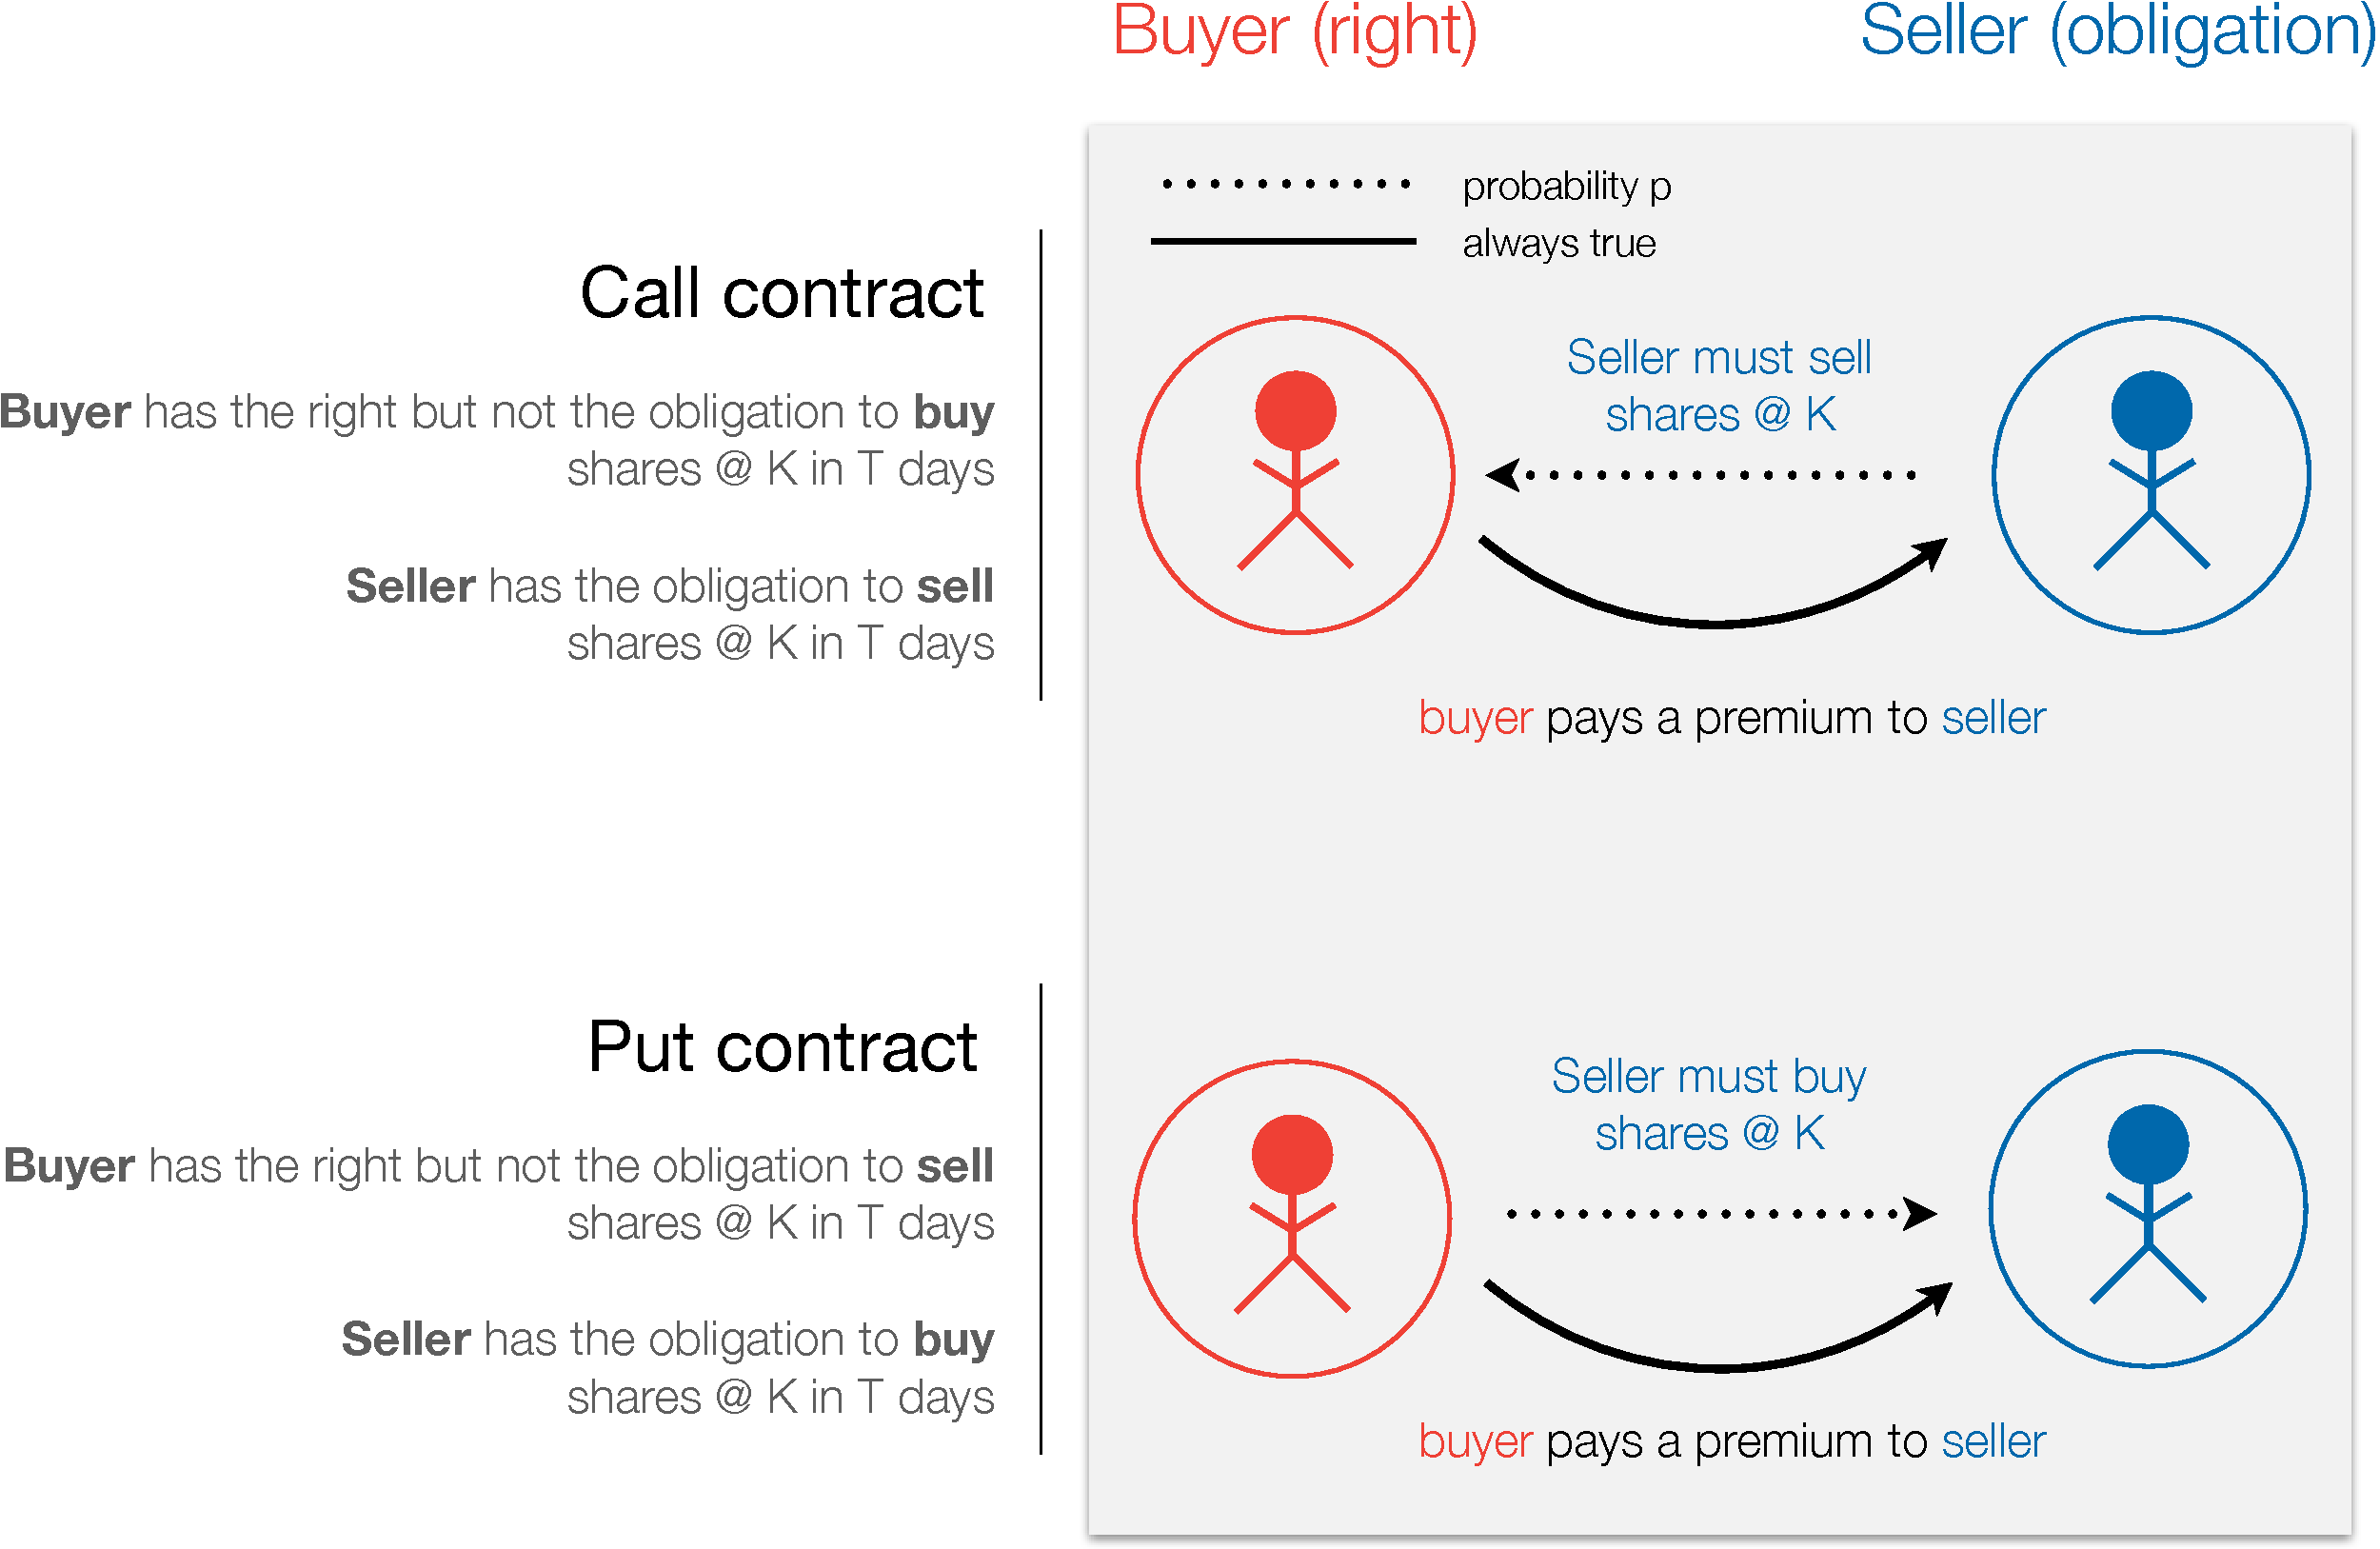
\includegraphics[width=0.85\textwidth]{./figs/Fig-Options-Table-Schematic.pdf}
    \caption{Schematic of call and put options contracts. The buyer pays a premium to the seller for the right, but 
	not the obligation to transact in the future, where the contract describes the transaction parameters.}\label{fig:options-schematic}
\end{figure}

\subsection{Call}
A \texttt{call} contract gives the holder (buyer) the right, but not the obligation, to purchase a specified asset, 
such as stocks, commodities, or currencies, to their counterparty (contract seller). 
Let's consider stock as the underlying asset. A single standard options contract controls 100 shares of stock. 
From the buyer's perspective, call contracts allow an investor to benefit from the upside price movement of a stock without purchasing the stock.
Further, call options (again from the buyer's perspective) have limited downside risk, i.e., the maximum amount the holder of the call option can lose 
is the premium paid for the option. Finally, call options are a mechanism to purchase shares of stock at the strike price of $K$ instead of the market price of $S$. 
On the other hand, from the seller's perspective, the main objective of selling a call contract is to collect the premium $\mathcal{P}$. 
Call contracts also allow the seller to benefit from downward price movement without purchasing shares of stock (in the case of a naked call).
However, for a seller, call options have unlimited upside risk; 
Thus, call options are often only sold by investors who already own the required number of shares of stock 
(known as a \href{https://www.investopedia.com/terms/c/coveredcall.asp}{covered call position}. 
Finally, call options offer the seller the opportunity to sell shares of stock at the strike price of $K$ instead of the market price of $S$.

\subsection{Put}
A \texttt{put} contract gives the holder (buyer) the right, but not the obligation, to sell a specified asset, 
such as stocks, commodities, or currencies, at a specified price to their counterparty (contract seller). 
Let's consider stock as the underlying asset. A single standard put contract controls 100 shares of stock.
From the buyer's perspective, put contracts allow an investor to benefit from the downward price movement of a stock without purchasing the stock. 
Further, put options (again from the buyer's perspective) have limited downside risk, i.e., the maximum amount the put option holder can lose is the premium paid for the option. 
Finally, put contracts are a mechanism to sell shares of stock at the strike price of $K$ instead of the market price of $S$. 
From the seller's perspective, the motivation for selling a put contract is to collect the premium $\mathcal{P}$. 
Put contracts also allow the seller to benefit from the price movement to the upside without purchasing shares.
However, for a seller, put options have unlimited downside risk; 
thus, put options are often only sold by investors who have set aside the required capital to purchase the required number of shares of stock 
(known as a \href{https://www.fidelity.com/learning-center/investment-products/options/know-about-cash-covered-puts}{cash-secured put position}).
Finally, put options offer the seller the opportunity to buy shares of a firm at the strike price of $K-\mathcal{P}$ instead of the market price of $S$.

\begin{concept}[Jargon: Long and Short Contracts]\label{concept:long-short-contracts}

	\textbf{Long contracts}: Instead of saying the \texttt{call} (or \texttt{put})) contract holder or buyer, you may sometimes hear the term \texttt{long call} (or \texttt{long put}) to denote a person has purchased a \texttt{call} (or \texttt{put}) contract.
	Thus, a person who buys an options contract is said to be \texttt{long} the \texttt{call} (or \texttt{put}) contract.
	
	\vspace{0.01in}
	\noindent\textbf{Short contracts}: On the other hand, instead of saying the \texttt{call} (or \texttt{put}) contract seller, you may hear the term \texttt{short call} (or \texttt{short put}) to denote a person has sold a \texttt{call} (or \texttt{put}) contract.
	Thus, a person who sells an options contract is said to be \texttt{short} the contract.
\end{concept}

\subsection{Payoff and Profit Diagrams for Long Contracts}
Unlike equity, e.g., shares of a stock or ETF, which have a linear payoff profile, both long and short options contracts have a nonlinear payoff profile depending on the price of the underlying asset at expiration, 
the strike price of the contract, the premium paid for the contract, and the type of contract (call or put).
For now, let's focus on long contracts, i.e., the buyer of the contract.

\subsubsection*{Call Options}
The payoff per share at expiration at time $t = T$ for a \texttt{call} option is:
\begin{equation}
V_{c}(K,S(T)) = \max\left(S(T) - K,~0\right)
\end{equation}
where $K$ denotes the strike price and $S(T)$ is the share price at expiration. 
The \texttt{seller} charges the \texttt{buyer} a premium at time $t=0$ (now), which we denote as $\mathcal{P}_{c}(K,S(0))$, for each contract.
Thus, the buyer's profit per share at expiration is the contract payoff minus the contract premium:
\begin{equation}
P_{c}(K,S(T)) = V_{c}(K,S(T)) -  \mathcal{P}_{c}(K,S(0))
\end{equation}
where $P_{c}(K,S(T)) = 0$ denotes the breakeven point for the buyer. 
Substituting the payoff and profit expressions into the breakeven equation, 
gives the breakeven share price $\mathcal{B}_{c}$ at expiration for the buyer 
of the \texttt{call} contract:
\begin{equation}
\mathcal{B}_{c} = K + \mathcal{P}_{c}(K,S(0))
\end{equation}
Thus, the share price at expiration must exceed the sum of the strike price and the premium for the buyer to make a profit.
An example payoff, profit, and breakeven diagram for a \texttt{call} contract from the buyer's perspective 
is shown in Fig. \ref{fig:call-payoff-profit-breakeven-diagram}.  
\begin{figure}[ht]
    \centering
    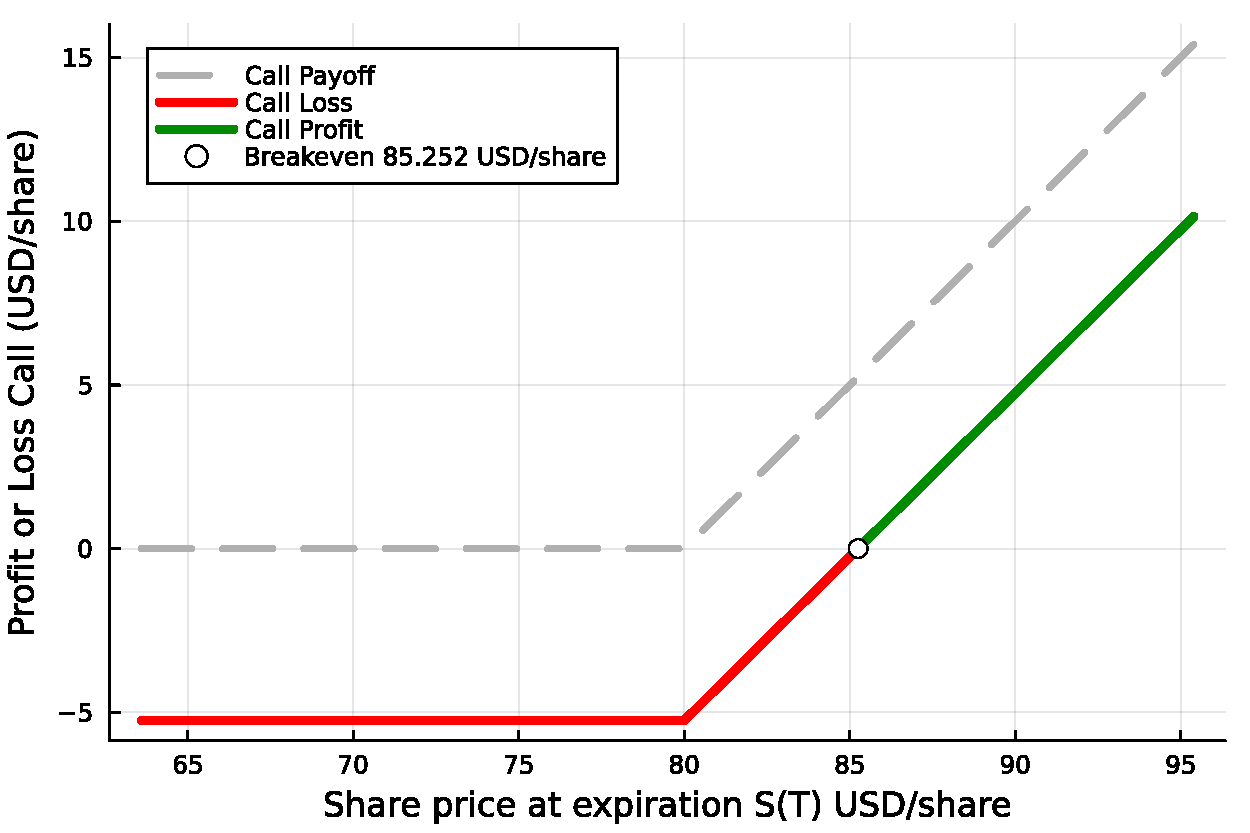
\includegraphics[width=0.65\textwidth]{./figs/Fig-Example-Call-K80-62DTE.pdf}
    \caption{Schematic of the payoff, profit and breakeven for a \texttt{long call} 
	contract. The gray dashed line denotes the payoff at expiration for the buyer.
	The red line denotes share prices at expiration that result in a loss for the buyer, 
	while the green line denotes share prices at expiration that result in a profit for the buyer.
	Parameters: the \texttt{call} 
	contract strike price is $K$ = 80 USD/share and the premium $\mathcal{P}_{c}$ = 5.25 USD/share.}\label{fig:call-payoff-profit-breakeven-diagram}
\end{figure}

% we can construct the payoff and profit diagrams for a call option (Fig. \ref{fig:call-option-payoff-profit}).
% The premium (cost) for each contract is governed by:
% \begin{equation*}
% \mathcal{P}_{c}(K,S(0))\geq\mathbb{E}\Bigl(\mathcal{D}^{-1}_{T,0}(\bar{r})\cdot{V_{c}}(K,S(T))\Bigr)
% \end{equation*}
% where $\mathcal{D}_{T,0}(\bar{r})$ denotes the risk neutral discount factor computed between purchase and contract expiration.

\subsubsection*{Put Options}
The payoff per share at expiration for a put option contract is given by:
\begin{equation}
V_{p}(K,S(T)) = \max\left(K - S(T),~0\right)
\end{equation}
where $K$ denotes the strike price and $S(T)$ is the share price at expiration. 
The \texttt{seller} charges the \texttt{buyer} a premium $\mathcal{P}_{p}(K,S(0))$ for each contract.
The buyer's profit per share at expiration is the payoff minus the contract premium:
\begin{equation}
P_{p}(K,S(T)) = V_{p}(K,S(T)) -  \mathcal{P}_{p}(K,S(0))
\end{equation}
where $P_{p}(K,S(T)) = 0$ denotes the breakeven point for the buyer. 
Substituting the payoff and profit expressions into the breakeven equation gives the breakeven share price $\mathcal{B}_{p}$ at expiration for the buyer 
of the \texttt{put} contract:
\begin{equation}
\mathcal{B}_{p} = K - \mathcal{P}_{p}(K,S(0))
\end{equation}
Thus, the share price at expiration must fall below the strike price minus the premium for the buyer of the \texttt{put} 
contract to make a profit.

\begin{figure}[ht]
    \centering
    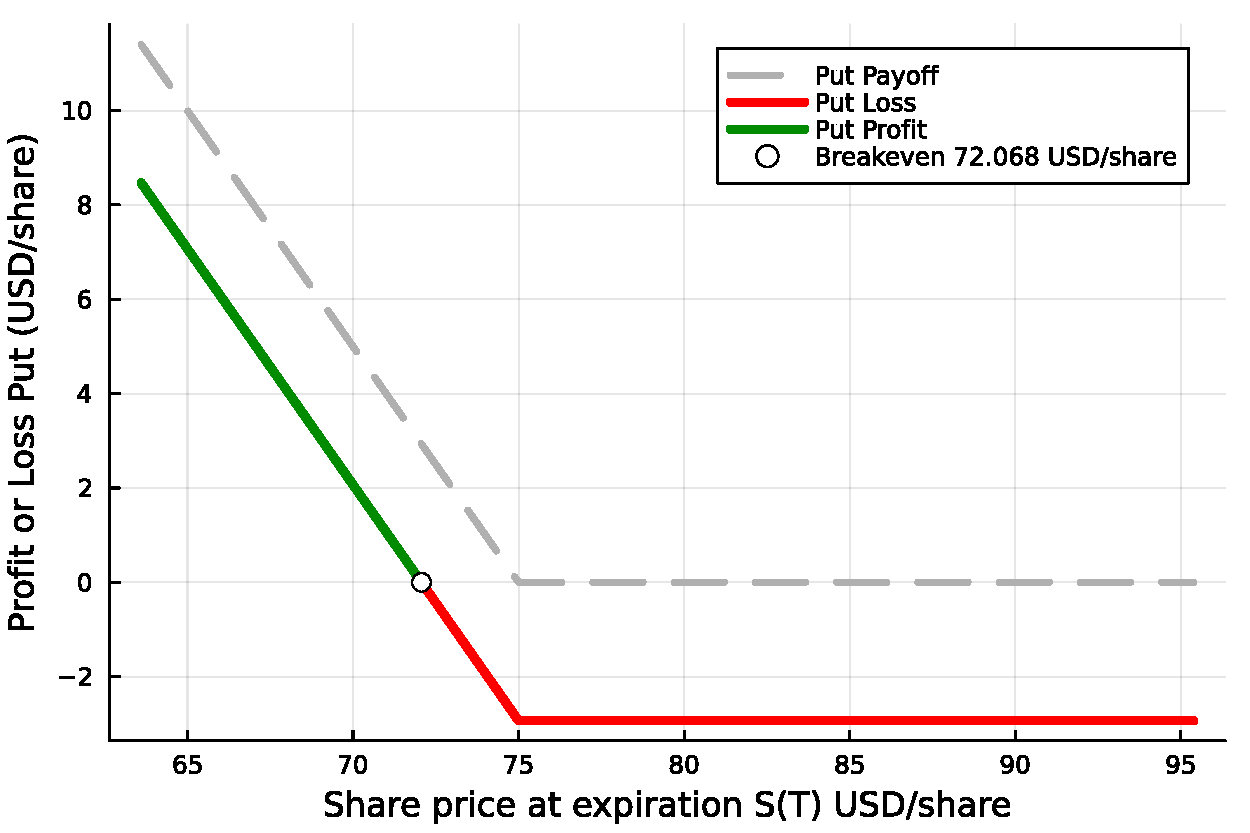
\includegraphics[width=0.65\textwidth]{./figs/Fig-Example-Put-K75-62DTE.pdf}
    \caption{Schematic of the payoff, profit and breakeven for a \texttt{long call} 
	contract. The gray dashed line denotes the payoff at expiration for the buyer.
	The red line denotes share prices at expiration that result in a loss for the buyer, 
	while the green line denotes share prices at expiration that result in a profit for the buyer.
	Parameters: the \texttt{put} 
	contract strike price is $K$ = 75 USD/share and a midpoint of premium $\mathcal{P}_{c}$ = 2.93 USD/share.}\label{fig:put-payoff-profit-breakeven-diagram}
\end{figure}

% The premium (cost) for a put contract is governed by:
% \begin{equation}
% \mathcal{P}_{p}(K,S(0))\geq\mathbb{E}\Bigl(\mathcal{D}^{-1}_{T,0}(\bar{r})\cdot{V_{p}}(K,S(T))\Bigr)
% \end{equation}
% where $\mathcal{D}_{T,0}(\bar{r})$ denotes the risk neutral discount factor computed between purchase and expiration.

\subsection{European Contracts Premiums}
An option's premium is the price the buyer pays the seller for the right to buy or sell an underlying asset at a specified price.
There are many methods to compute the premium of an options contract, but the most widely used method (by far) is the Black-Scholes-Merton (BSM) model (and its extensions).
The BSM model has a closed-form solution, i.e., a mathematical expression that can be evaluated directly. Thus, it is computationally efficient.
Alternatively, the premium of an options contract can be computed using numerical methods, such as binomial trees or Monte Carlo simulation.
Let's consider the BSM model first, and then we'll explore a Monte Carlo method to price European calls and put contracts.

\subsubsection*{The Black-Scholes-Merton (BSM) Model}
The Black-Scholes-Merton model is used to compute the premium of European-style options contracts \cite{BlackScholes1973};
Robert C. Merton, Myron S. Scholes, and Fischer Black won the \href{https://www.nobelprize.org/prizes/economic-sciences/1997/press-release/}{Nobel Prize in Economics in 1997} for their work on this model.
The model assumes that the underlying asset's price follows a geometric Brownian motion with constant drift and volatility, where the drift is the risk-free interest rate, i.e., we evaluate the option using a risk-neutral pricing paradigm.
Further, the model assumes that the risk-free interest rate is constant and that the underlying stock does not pay dividends (although the model can be modified to include dividends).
Under these assumptions, the price of the option can be computed using the Black-Scholes-Merton pricing formula, which is the parabolic partial differential equation:
\begin{eqnarray}\label{eqn:BSM-pde}
	\frac{\partial{V}}{\partial{t}} + \frac{1}{2}\sigma^{2}S^{2}\frac{\partial^{2}V}{\partial{S}^{2}} & = & \bar{r}V - rS\frac{\partial{V}}{\partial{S}}  \\
	\frac{dS}{S} & = & \bar{r}\,dt + \sigma\,{dW}\\
	V(T,S) & = & K(S)
\end{eqnarray}
where $V(t, S)$ is the price of the option, $S$ is the price of the underlying asset (governed by the risk-neutral geometric Brownian motion model), 
$K(S)$ is the payoff of the option at expiration, $T$ is the expiration date, $t$ is time, 
$\bar{r}$ is the risk-free interest rate, and $\sigma$ is the volatility of the underlying asset.
$t$ is time, $r$ is the risk-free interest rate, and $\sigma$ is the volatility of the underlying asset.
While we could solve the partial differential equation \ref{eqn:BSM-pde} directly, it is more common to use the closed-form solution of the Black-Scholes-Merton pricing formula.

The price of a European \texttt{call} option is given by Definition \ref{defn:BSM-call-closed-form}:
\begin{definition}[Black-Scholes-Merton Pricing Formula for a European Call Option]\label{defn:BSM-call-closed-form}
The Black-Scholes-Merton pricing formula for a European \texttt{call} option is given by the expression:
\begin{equation}
	\mathcal{P}_{c}(K,S(0)) = N(d_{+})S(0) - N(d_{-})K\mathcal{D}^{-1}_{T,0}(\bar{r})
\end{equation}
where $N(\dots)$ denotes the standard normal cumulative distribution function, $S(0)$ is the price of the underlying asset at time $t=0$ (when we are evaluating the option),
$K$ is the strike price of the contract, and $\mathcal{D}^{-1}_{T,0}(\bar{r})$ is the discount factor from time $t=0$ to time $T$ evaluated at the risk-free interest rate $\bar{r}$.
The arguments of the normal cumulative distribution function are given by:
\begin{eqnarray}
d_{+} & = & \frac{1}{\sigma\sqrt{T}}\left[\ln(\frac{S_{\circ}}{K}) + (\bar{r}+\frac{\sigma^{2}}{2})T\right] \\
d_{-} & = & d_{+} - \sigma\sqrt{T}
\end{eqnarray}
\end{definition}
while the price of a European \texttt{put} option is given by Definition \ref{defn:BSM-put-closed-form}:
\begin{definition}[Black-Scholes-Merton Pricing Formula for a European Put Option]\label{defn:BSM-put-closed-form}
The Black-Scholes-Merton pricing formula for a European \texttt{put} option is given by the expression:
\begin{equation}
\mathcal{P}_{p}(K,S(0)) = N(-d_{-})\cdot{K}\cdot\mathcal{D}^{-1}_{T,0}(\bar{r}) - N(-d_{+})\cdot{S}(0)
\end{equation}
where $N(\dots)$ denotes the standard normal cumulative distribution function, 
$S(0)$ is the price of the underlying asset at time $t=0$ (when we are evaluating the option),
$K$ is the strike price of the contract, and $\mathcal{D}^{-1}_{T,0}(\bar{r})$ is the discount factor from time $t=0$ to time $T$ evaluated at the risk-free interest rate $\bar{r}$.
The arguments of the normal cumulative distribution function are given by:
\begin{eqnarray}
d_{+} & = & \frac{1}{\sigma\sqrt{T}}\left[\ln(\frac{S_{\circ}}{K}) + (\bar{r}+\frac{\sigma^{2}}{2})T\right] \\
d_{-} & = & d_{+} - \sigma\sqrt{T}
\end{eqnarray}
\end{definition}

\subsubsection*{Monte Carlo Simulation for European Contracts}
Alternatively, we can compute the premium of the European options contract using a Monte Carlo simulation.
The premium $\mathcal{P}_{\star}(K,S(0))$ the buyer is willing to pay for a European \texttt{call} (or \texttt{put}) contract with an expiration $T$-periods from today is given by the equality:
\begin{equation}\label{eqn:BSM-premium-equality-mc}
\mathcal{P}_{\star}(K,S(0)) = \mathbb{E}\Bigl(\mathcal{D}^{-1}_{T,0}(\bar{r})\cdot{V_{\star}}(K,S(T))\Bigr)
\end{equation}
where $\mathcal{D}_{T,0}(\bar{r})$ denotes the risk-neutral discount factor computed between purchase and expiration using the discount rate $\bar{r}$, $V_{\star}(K, S(T))$ is the payoff of the contract $\star$ at expiration, $S(T)$ is the share price at expiration, $K$ is the strike price of the contract, and $S(0)$ is the share price at time $t=0$ (now) when we are purchasing the contract. Equation \ref{eqn:BSM-premium-equality-mc} says the premium an investor is willing to pay for a contract is the expected value of the discounted future payoff from the contract. This is true for both \texttt{call} and \texttt{put} contracts. But why is this true?

\begin{concept}[Excerise risk]
Because the buyer can \textit{only} exercise the contract at expiration, a fair premium for a European options contract must be the expected value of the discounted future payoff. A rational investor will only pay as much for a contract as they hope to make from the contract. 
They would lose money on average if they paid more than the expected value of the future payoff.
\end{concept}
The expectation in Eqn. \ref{eqn:BSM-premium-equality-mc} can be computed using Monte Carlo simulation.
We can compute the premium of a European \texttt{call} or \texttt{put} contract by simulating the future share price $S(T)$ at contract expiration
using a geometric Brownian motion model and then directly computing the expected value of the discounted future payoff from the contract 
using the simulated samples paths. 

\subsection{Summary}
In this module, we introduced the concept of derivatives and focused on European-style options contracts. 
We introduced the two types of options contracts: \texttt{call} and \texttt{put} contracts. 
A \texttt{call} contract gives the holder the right, but not the obligation, to buy an underlying asset at a specified price (strike) 
on or before a future date (expiration). On the other hand, a \texttt{put} contract gives the holder the right, but not the obligation, 
to sell an underlying asset at a specified price (strike) on or before a future date (expiration). 
We introduced the payoff and profit diagrams for both types of contracts and discussed 
the Black-Scholes-Merton model for computing the premium of European contracts. 
Finally, we discussed how the premium of a European contract can be calculated using Monte Carlo simulation.

\section{American Style Options Contracts}
In the previous section, we introduced European-style options contracts. Here, we'll introduce American-style options contracts.
The key difference between an American and European call contracts is the time at which the option can be exercised.
An American call contract can be exercised at any time on or before the expiration date, while a European call contract can only be exercised at expiration.
The extra flexibility of an American call contract comes at a cost, and thus the premium for an American call contract is at least that of a European call contract.

\subsection{American Call Options}
The payoff per share at expiration for a call option is:
\begin{equation*}
V_{c}(K,S(T)) = \max\left(S(T) - K,~0\right)
\end{equation*}
where $K$ denotes the strike price and $S(T)$ is the share price at expiration. 
The \texttt{seller} charges the \texttt{buyer} a premium $\mathcal{P}_{c}(K,S(0))$ for each contract.
The buyer's profit per share at expiration is the payoff minus the contract premium:
\begin{equation*}
P_{c}(K,S(T)) = V_{c}(K,S(T)) -  \mathcal{P}_{c}(K,S(0))
\end{equation*}
The premium (cost) for each contract is governed by:
\begin{equation*}
\mathcal{P}_{c}(K,S(0))\geq\mathbb{E}\Bigl(\mathcal{D}^{-1}_{T,0}(\bar{r})\cdot{V_{c}}(K,S(T))\Bigr)
\end{equation*}
where $\mathcal{D}_{T,0}(\bar{r})$ denotes the risk neutral discount factor computed between purchase and contract expiration.

\begin{figure}[ht]
    \centering
    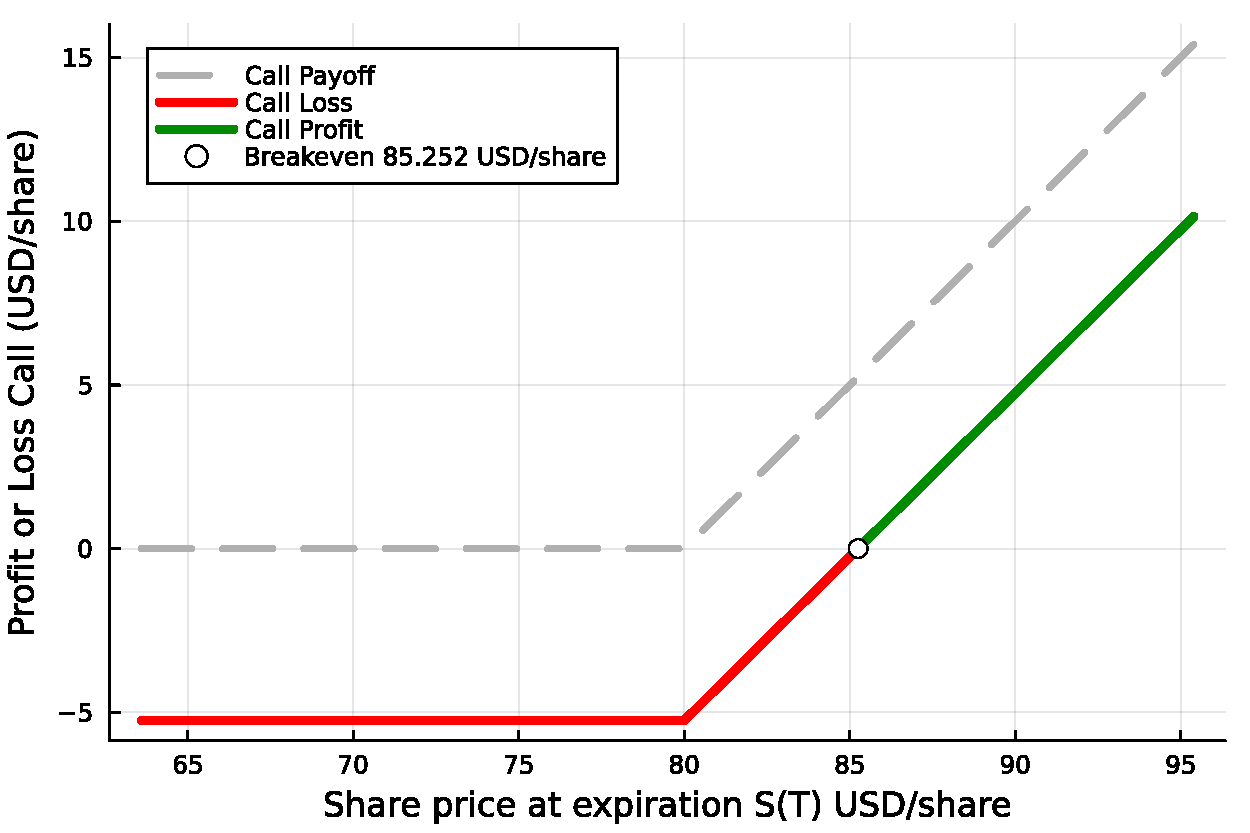
\includegraphics[width=0.65\textwidth]{./figs/Fig-Example-Call-K80-62DTE.pdf}
    \caption{Schematic of the payoff, profit and breakeven for a \texttt{long call} 
	contract. The gray dashed line denotes the payoff at expiration for the buyer.
	The red line denotes share prices at expiration that result in a loss for the buyer, 
	while the green line denotes share prices at expiration that result in a profit for the buyer.
	Parameters: the \texttt{call} 
	contract strike price is $K$ = 80 USD/share and the premium $\mathcal{P}_{c}$ = 5.25 USD/share.}\label{fig:call-payoff-profit-breakeven-diagram}
\end{figure}

\subsection{American Put Options}
The payoff per share at expiration for a put option contract is given by:
\begin{equation*}
V_{p}(K,S(T)) = \max\left(K - S(T),~0\right)
\end{equation*}
where $K$ denotes the strike price and $S(T)$ is the share price at expiration. 
The \texttt{seller} charges the \texttt{buyer} a premium $\mathcal{P}_{p}(K,S(0))$ for each contract.
The buyer's profit per share at expiration is the payoff minus the contract premium:
\begin{equation*}
P_{p}(K,S(T)) = V_{p}(K,S(T)) -  \mathcal{P}_{p}(K,S(0))
\end{equation*}
The premium (cost) for a put contract is governed by:
\begin{equation*}
\mathcal{P}_{p}(K,S(0))\geq\mathbb{E}\Bigl(\mathcal{D}^{-1}_{T,0}(\bar{r})\cdot{V_{p}}(K,S(T))\Bigr)
\end{equation*}
where $\mathcal{D}_{T,0}(\bar{r})$ denotes the risk neutral discount factor computed between purchase and expiration.

\begin{figure}[ht]
    \centering
    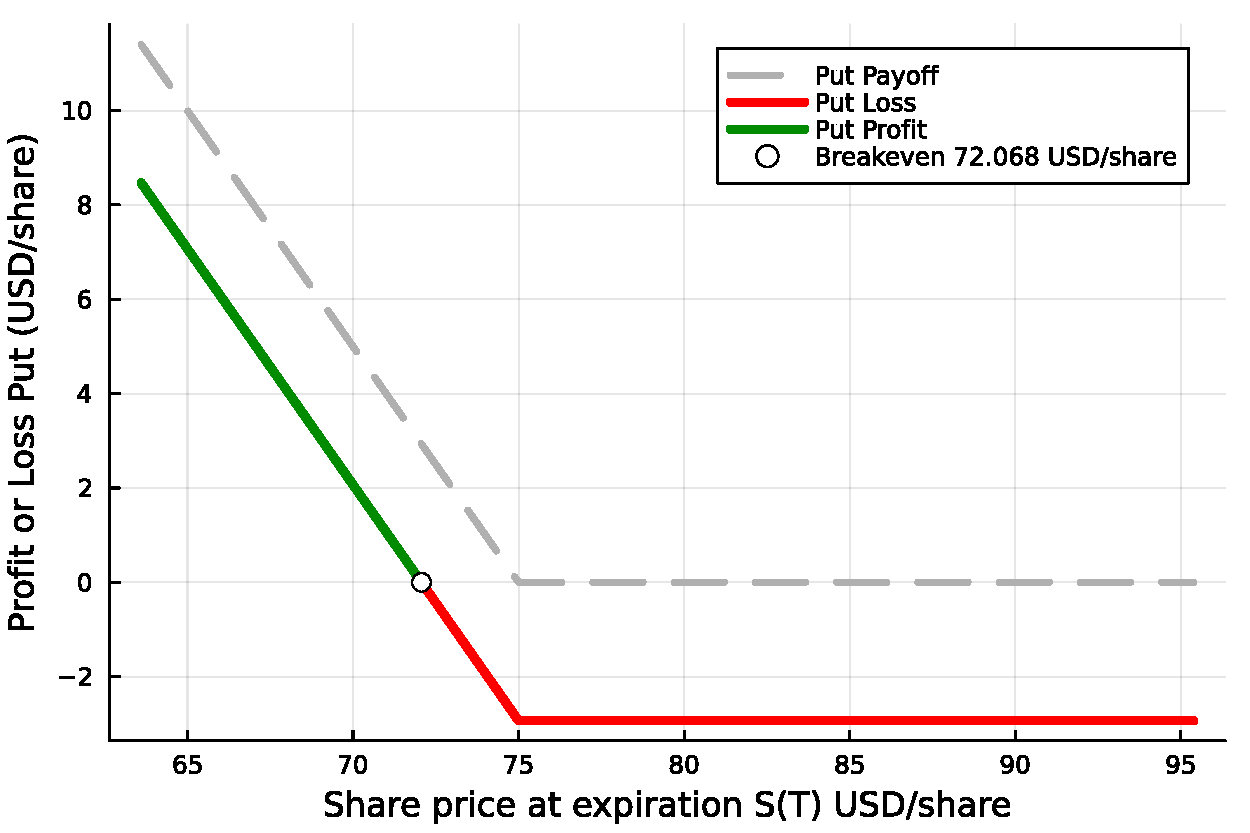
\includegraphics[width=0.65\textwidth]{./figs/Fig-Example-Put-K75-62DTE.pdf}
    \caption{Schematic of the payoff, profit and breakeven for a \texttt{long call} 
	contract. The gray dashed line denotes the payoff at expiration for the buyer.
	The red line denotes share prices at expiration that result in a loss for the buyer, 
	while the green line denotes share prices at expiration that result in a profit for the buyer.
	Parameters: the \texttt{put} 
	contract strike price is $K$ = 75 USD/share and a midpoint of premium $\mathcal{P}_{c}$ = 2.93 USD/share.}\label{fig:put-payoff-profit-breakeven-diagram}
\end{figure}


\subsection{Summary}
In this section we introduced American style call contracts.
A \texttt{call} contract gives the holder the right, but not the obligation, to buy an underlying asset at a specified price (strike) on or before a future date (expiration).
We introduced the payoff and profit diagrams for \texttt{call} contracts.
On the other hand, a \texttt{put} contract gives the holder the right, but not the obligation, to sell an underlying asset at a specified price (strike) on or before a future date (expiration).

\section{American-Style Composite Contracts at Expiration}
Composite options contracts are financial instruments comprising two or more individual options contracts. 
The payoff and profit of a composite contract at expiration is the sum of the values of the individual contracts. 
The advantage of constructing composite contracts is that they can be used to construct complex payoffs and profit strategies 
from simple contract components. In this module, we will analyze composite contracts at expiration, 
where the composite contract comprises two or more American-style options.

\subsection{General Composite Contract Formulation}
Call and put contracts can be combined to develop composite contract structures with interesting payoff diagrams. Let $\mathcal{C}$ be a composite contract with $d$ legs (individual contracts) where each leg is written for the same underlying asset \texttt{XYZ} and the same expiration date. 
Then, the payoff of the composite contract $\hat{V}(S(T),K_{1},\dots,K_{d})$ at time $T$ (expiration) is given by:
\begin{equation}
\hat{V}(S(T),K_{1},\dots,K_{d}) = \sum_{i\in\mathcal{C}}\theta_{i}\cdot{n_{i}}\cdot{V_{i}(S(T),K_{i}})
\end{equation}
where $K_{i}$ denotes the strike price of contract $i$, $\theta_{i}$ denotes the contract orientation $i$: $\theta_{i}=-1$ if contract $i$ is short (sold), 
otherwise $\theta_{i}=1$, and the quantity $n_{i}$ denotes the copy number of contract $i$.
The profit of the composite contract $\hat{P}$ at time $T$ (expiration) is given by:
\begin{equation}
\hat{P}(S(T),K_{1},\dots,K_{d}) = \sum_{i\in\mathcal{C}}\theta_{i}\cdot{n}_{i}\cdot{P}_{i}(S(T),K_{i})
\end{equation}
where $P_{i}(S(T),K_{i})$ denotes the profit of contract $i$. 
Finally, the profit for a contract of type $\star$ is given by:
\begin{equation}
P_{\star}(K,S(T)) = {V}_{\star}(K,S(T)) -  \mathcal{P}_{\star}(K,S(0))
\end{equation}
where $\mathcal{P}_{\star}(K,S(0))$ denotes the premium of contract $\star$, and ${V}_{\star}(K,S(T))$ 
denotes the payoff of contract $\star$ at expiration.

\subsection{Defined-Risk Directional Composite Contracts}
Directional composite contracts make a directional assumption about the underlying asset's price movement and can be opened for a credit or debit.
A common directional composite contract is a \textit{spread}.

\subsubsection*{Put Vertical Spread}
A \texttt{put} vertical spread is constructed by combining 2 $\times$ \texttt{put} contracts; a short \texttt{put} contract generates income while a \texttt{long} put contract controls downside risk.  
Let contract $j$ have a strike price of $K_{j}$ and premium $\mathcal{P}_{j}$. 
The share price at expiration is given by $S$. 
Finally, let contract 1 be the short \texttt{put} leg $\theta_{1} = -1$ and contract 2 be the long \texttt{put} leg $\theta_{2} = 1$. 
Then, the profit for a single \texttt{put} vertical spread at expiration is given by:
\begin{equation}
\hat{P} = -P_{1}+P_{2}
\end{equation}
which, after substitution of the profit functions for a put contract, gives:
\begin{equation}
\hat{P} = \left(K_{2} - S\right)^{+} - \left(K_{1} - S\right)^{+} + \left(\mathcal{P}_{1} - \mathcal{P}_{2}\right)
\end{equation}
where $V_{p} = (K-S)^{+}=\max(K-S,0)$ is the payoff function for a \texttt{put} contract. 
The first term is the net payout of the two legs of the spread, while the second term is the net cost of the two contracts. 
The maximum possible profit, loss, and breakeven conditions are given by:
\begin{itemize}
\item{The maximum possible profit of $\left(\mathcal{P}_{1} - \mathcal{P}_{2}\right)$ will occur when $S\geq{K_{1}}$.}
\item{The maximum possible loss of $K_{2} - K_{1} + \left(\mathcal{P}_{1} - \mathcal{P}_{2}\right)$ will occur when $S\leq{K_{2}}$.}
\item{The vertical put spread will breakeven when $S =  K_{1}+\left(\mathcal{P}_{2} - \mathcal{P}_{1}\right)$.}
\end{itemize}

\subsubsection*{Bearish call credit spread}
A bear \texttt{call} credit spread is an options strategy used 
when a trader expects a decline in the price of the underlying asset. 
Assume the initial share price of the underlying asset is $S_{o}$ (when we are opening the trade).
For this trade, we sell a \texttt{call} contract at $K_{1}<S_{o}$ for $\mathcal{P}_{1}$, 
and buy a \texttt{call} contract at $K_{2}>S_{o}$ for $\mathcal{P}_{2}$. The profit function 
for the bear \texttt{call} credit spread is given by:
\begin{equation}
\hat{P} = (S-K_{2})^{+} - (S-K_{1})^{+} + (\mathcal{P}_{1}-\mathcal{P}_{2})
\end{equation}
where $V_{c} = (S-K)^{+}=\max(S-K,0)$ is the payoff function for a \texttt{call} contract. 
The first two terms are the net payout of the two legs of the spread, while the last term is the net cost of the two contracts. 
The maximum possible profit, loss, and breakeven conditions are given by:
\begin{itemize}
\item{The maximum possible profit of $\left(\mathcal{P}_{1} - \mathcal{P}_{2}\right)$ will occur when $S\leq{K_{1}}$.}
\item{The maximum possible loss of $\left(\mathcal{P}_{1} - \mathcal{P}_{2}\right) -(K_{2} - K_{1})$ will occur when $S\geq{K_{2}}$.}
\item{The bear \texttt{call} spread will breakeven when $S =  K_{1}+\left(\mathcal{P}_{1} - \mathcal{P}_{2}\right)$.}
\end{itemize}

\subsection{Neutral Composite Contracts}
Neutral composite contracts make no directional assumption about the price movement of the underlying asset and can be opened for credit or debit.
Two common directional composite contracts are the \textit{straddle} and the \textit{strangle}.	

\subsubsection*{Straddles}
A \href{https://www.investopedia.com/terms/s/straddle.asp}{straddle} is a neutral strategy constructed by simultaneously buying (or selling) 
a put and a call option on the same underlying asset \texttt{XYZ}, with the same expiration and the same strike price (Fig. \ref{fig:options-short-straddle-profit}). 

\begin{figure}[h]
    \centering
    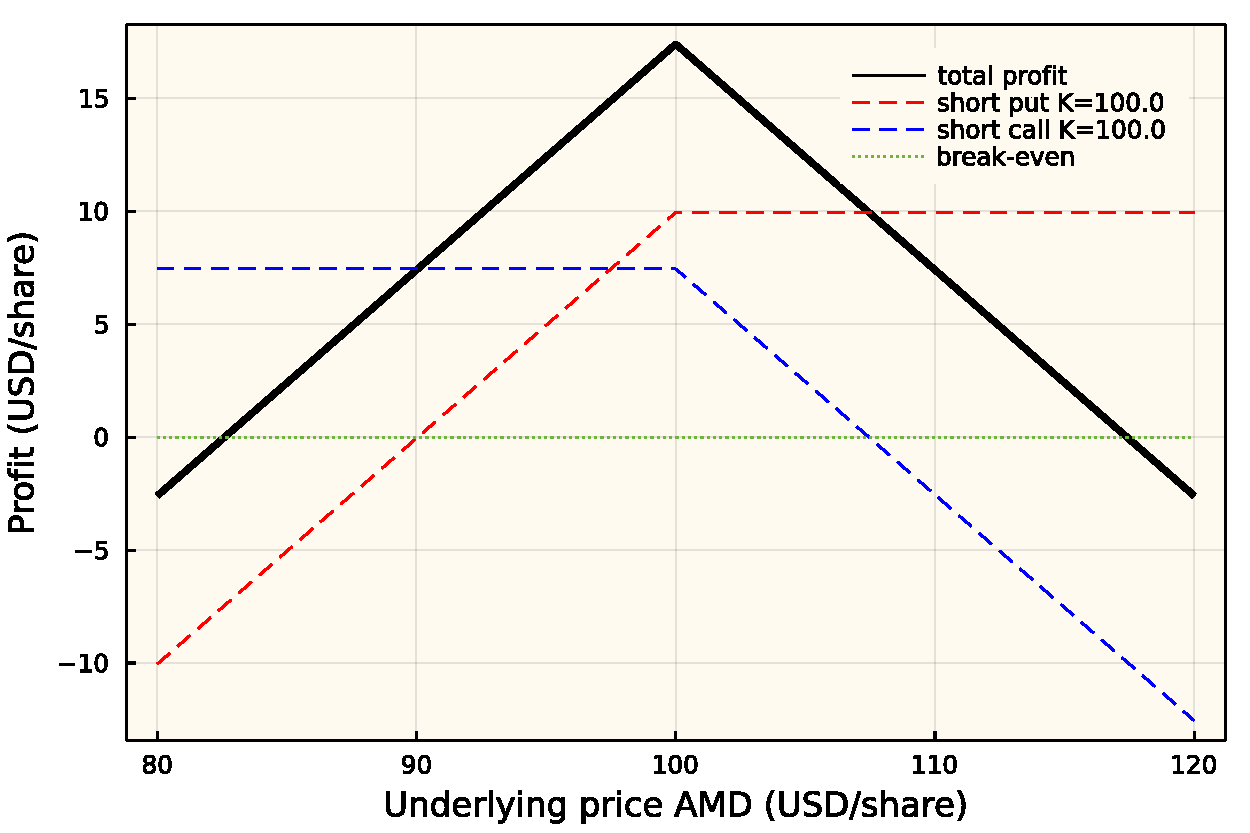
\includegraphics[width=0.75\textwidth]{./figs/Fig-AMD-Profit-Short-Straddle.pdf}
    \caption{Schematic of the profit for a short straddle trade written for Advanced Micro Devices, Inc. with ticker symbol \texttt{AMD}.
	A short straddle is a neutral strategy constructed by simultaneously selling a put and a call option on the same underlying asset \texttt{AMD}, with the same expiration and strike price.
	Conversely, a long straddle is a neutral strategy constructed by simultaneously buying a put and a call option on the same underlying asset \texttt{AMD}, with the same expiration and strike price.
	A long straddle has the same breakeven points as a short straddle, but the profit and loss are reversed, i.e., the profit diagram is rotated around the breakeven line.
	Thus, a long straddle has a defined maximum loss and an unlimited maximum possible profit.
	}\label{fig:options-short-straddle-profit}
\end{figure}

Depending upon the choice of the strike prices and whether an investor buys or sells both legs, 
a \href{https://www.investopedia.com/terms/s/straddle.asp}{straddle} can be initiated as a credit or debit and potentially have undefined profit or loss.
Let $K_{j}$ denote the strike price of contract $j$ (USD/share), where the price of contract $j$ is $\mathcal{P}_{j}$ (USD/share). 
Further, let index $j=1$ denote the \texttt{put} contract, $j=2$ denote the \texttt{call} contract; 
for a straddle $K_{1}= K_{2}\equiv{K}$ (both legs have the same strike). The profit for a single straddle contract $\hat{P}$ at expiration is given by:
\begin{equation}
\hat{P} = \theta\cdot\left(P_{1}+P_{2}\right)
\end{equation}
where $\theta_{1}=\theta_{2}\equiv\theta$ denotes a direction parameter: $\theta=-1$ if each leg is sold (short),
$\theta=1$ otherwise. After substitution of the profit functions for a \texttt{put} and a \texttt{call} contract, the overall profit $\hat{P}$ for a \texttt{straddle} 
is given by:
\begin{equation}
\hat{P} = \theta\cdot\Bigl[(K-S)^{+}+(S-K)^{+}-(\mathcal{P}_{1}+\mathcal{P}_{2})\Bigr]
\end{equation}
where $V_{p} = (K-S)^{+}=\max(K-S,0)$ is the payoff function for the \texttt{put} contract, and $V_{c} = (S-K)^{+} = \max(S-K,0)$ is the payoff function for the \texttt{call} contract. 
The profit (or loss) of a straddle has three regimes given by:
\begin{equation}
\hat{P} = \begin{cases}
  \theta\cdot\Bigl[(S(T)-K)-\left(\mathcal{P}_{1}+\mathcal{P}_{2}\right)\Bigr]  & S(T)>K \\
  -\theta\cdot\Bigl[\mathcal{P}_{1}+\mathcal{P}_{2}\Bigr] & S(T)=K \\
    \theta\cdot\Bigl[(K-S(T))-\left(\mathcal{P}_{1}+\mathcal{P}_{2}\right)\Bigr] & S(T)<K
\end{cases}
\end{equation}
where $S(T)$ denotes the share price of the underlying asset at expiration. Finally, a straddle has two possible breakeven points denoted as $S^{+}$ and $S^{-}$:
\begin{equation}
	\mathcal{B}(T) = \begin{cases}
		S^{+} = K + \left(\mathcal{P}_{1}+\mathcal{P}_{2}\right) & S(T)>K \\
		S^{-} = K - \left(\mathcal{P}_{1}+\mathcal{P}_{2}\right) & S(T)<K
	\end{cases}
\end{equation}
where $S^{+}$ denotes the upper breakeven point, and $S^{-}$ denotes the lower breakeven point.

\subsubsection*{Strangles}
A \href{https://www.investopedia.com/terms/s/strangle.asp}{strangle} is a neutral strategy constructed by simultaneously buying (or selling)
a \texttt{put} and a \texttt{call} option on the same underlying asset \texttt{XYZ}, with the same expiration, but with different strike prices (Fig. \ref{fig:options-short-strangle-profit}).

\begin{figure}[h]
    \centering
    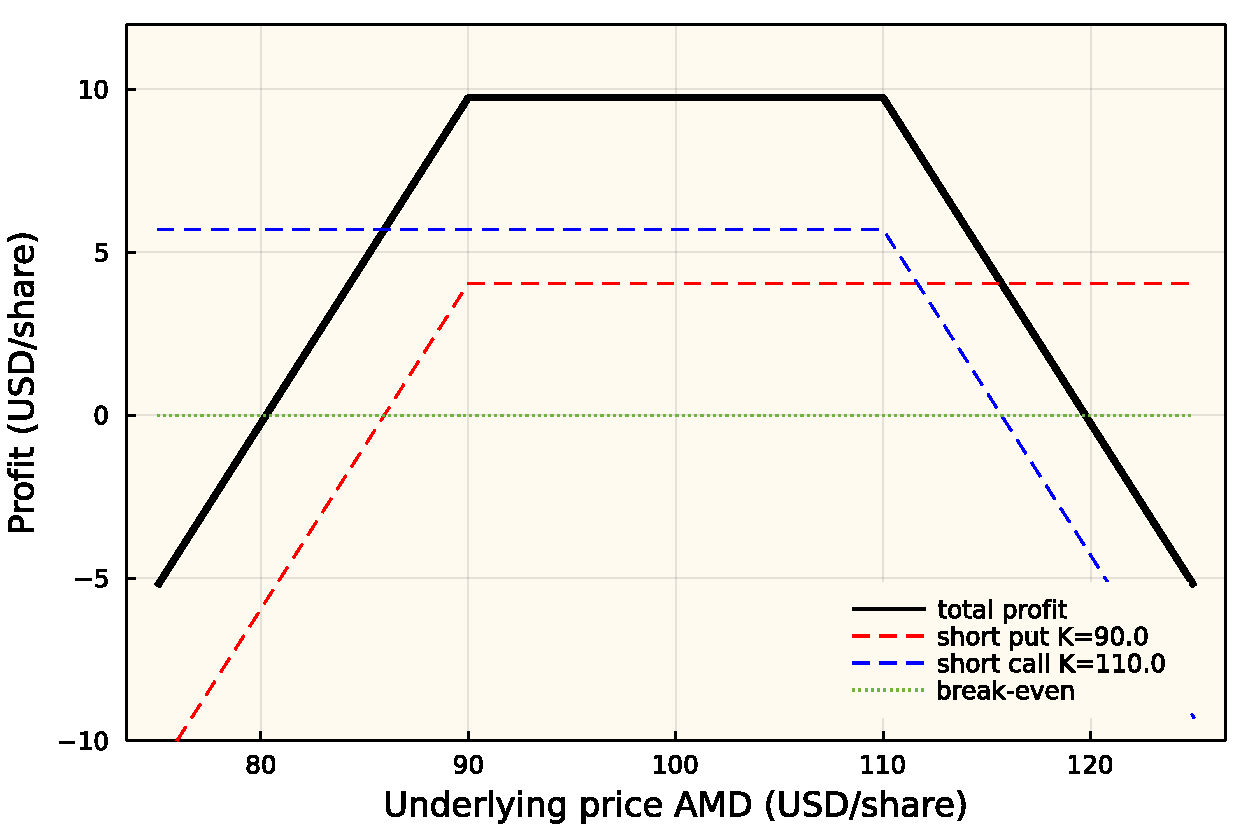
\includegraphics[width=0.75\textwidth]{./figs/Fig-AMD-Profit-Short-Strangle.pdf}
    \caption{Schematic of the profit for a short strangle trade written for Advanced Micro Devices, Inc. with ticker symbol \texttt{AMD}.
	A short strangle is a neutral, undefined risk strategy constructed by simultaneously selling a put and a call option on the same underlying asset \texttt{AMD}, with the same expiration but different strike prices.
	On the other hand, a long strangle is a neutral strategy constructed by simultaneously buying a put and a call option on the same underlying asset \texttt{AMD}, with the same expiration but different strike prices.
	A long strangle has the same breakeven points as a short strangle, but the profit and loss are reversed, i.e., the profit diagram is rotated around the breakeven line.
	Thus, a long strangle has a defined maximum loss and an undefined maximum possible profit.
	}\label{fig:options-short-strangle-profit}
\end{figure}

Depending upon the choice of the strike prices and whether an investor buys or sells both legs, a \href{https://www.investopedia.com/terms/s/strangle.asp}{strangle} 
can be initiated for a credit or debit and potentially have undefined profit or loss. Let $K_{j}$ denote the strike price of contract $j$ (USD/share), 
where the price of contract $j$ is $\mathcal{P}_{j}$ (USD/share). Further, let index $j=1$ denote the \texttt{put} contract, $j=2$ denote the \texttt{call} contract; 
for a strangle $K_{1}<K_{2}$. The profit for a single strangle contract $\hat{P}$ at expiration is given by:
\begin{equation}
\hat{P} = \theta\cdot\left(P_{1}+P_{2}\right)
\end{equation}
where $\theta_{1} = \theta_{2}\equiv\theta$ denotes a direction parameter: $\theta=-1$ if each leg is sold (short), $\theta=1$ otherwise. 
After substitution of the profit functions for a \texttt{put} and a \texttt{call} contract, the overall profit $\hat{P}$ for a \texttt{strangle} 
is given by:
\begin{equation}
\hat{P} = \theta\cdot\Bigl[(K_{1}-S)^{+}+(S-K_{2})^{+}-(\mathcal{P}_{1}+\mathcal{P}_{2})\Bigr]
\end{equation}
where $V_{p} = (K_{1}-S)^{+}=\max(K_{1}-S,0)$ is the payoff for the \texttt{put} contract, 
and $V_{c} = (S-K_{2})^{+} = \max(S-K_{2},0)$ is the payoff for the \texttt{call} contract. 
The profit (or loss) of a strangle has three regimes given by:
\begin{equation}
\hat{P} = \begin{cases}
  \theta\cdot\Bigl[(S(T)-K_{2})-\left(\mathcal{P}_{1}+\mathcal{P}_{2}\right)\Bigr]  & S(T)>K_{2} \\
  -\theta\cdot\Bigl[\mathcal{P}_{1}+\mathcal{P}_{2}\Bigr] & K_{1}\leq{S(T)}\leq{K_{2}} \\
  \theta\cdot\Bigl[(K_{1}-S(T))-\left(\mathcal{P}_{1}+\mathcal{P}_{2}\right)\Bigr] & S(T)<{K_{1}}
\end{cases}
\end{equation}
where $S(T)$ denotes the share price of the underlying asset at expiration. 
Finally, a strangle has two possible breakeven points denoted as $S^{+}$ and $S^{-}$:
\begin{equation}
	\mathcal{B}(T) = \begin{cases}
		S^{+} = K_{1} - \left(\mathcal{P}_{1}+\mathcal{P}_{2}\right) & S(T) > K_{2} \\
		S^{-} = K_{2} + \left(\mathcal{P}_{1}+\mathcal{P}_{2}\right) & S(T) < K_{1}
	\end{cases}
\end{equation}
where $S^{+}$ denotes the upper breakeven point, and $S^{-}$ denotes the lower breakeven point.

\subsubsection*{Iron Condor}
Iron Condors are examples of defined-risk neutral strategies, i.e., they make no directional assumption about the price movement of the underlying asset, 
and can be opened for credit or debit.
However, unlike straddles and strangles, iron condors have a defined maximum loss and maximum possible profit (Fig. \ref{fig:options-iron-condor-profit}).
An \href{https://www.investopedia.com/terms/i/ironcondor.asp}{iron condor} is a neutral defined risk position constructed 
by \textit{selling} a put (1) and call (2) options on the underlying asset \texttt{XYZ}, 
while simultaneously \textit{buying} a put (3) and call (4) options on \texttt{XYZ}. 
All the legs of an \href{https://www.investopedia.com/terms/i/ironcondor.asp}{iron condor} have the same underlying asset \texttt{XYZ}, 
and have the same expiration, but they have different strike prices where $K_{3}<K_{1}<K_{2}<K_{4}$. 
In particular, the two short options are sold with strikes on either side of the current share price $S_{o}$ of \texttt{XYZ}, 
with the short put strike price $K_{1}<S_{o}$ and the short call strike price $K_{2}>S_{o}$. 
Then, the long legs are purchased above and below the short strikes.  
Thus, an \href{https://www.investopedia.com/terms/i/ironcondor.asp}{iron condor} position has the character of a 
\href{https://www.investopedia.com/terms/s/strangle.asp}{strangle} combined with a vertical spread. 

\begin{figure}[h]
    \centering
    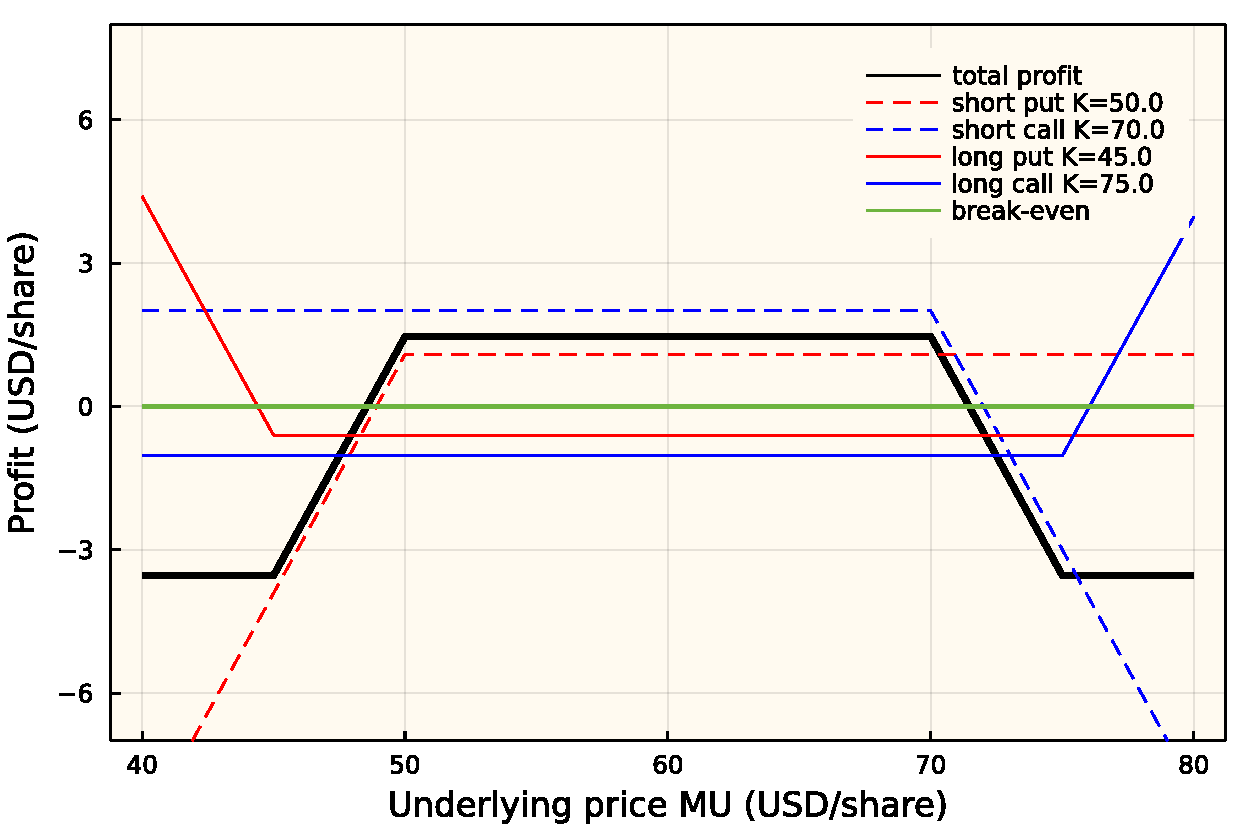
\includegraphics[width=0.75\textwidth]{./figs/Fig-MU-Profit-IronCondor.pdf}
    \caption{Schematic of the profit for an Iron Condor on Micron Technologies with ticker symbol \texttt{MU}.
	An iron condor is a neutral defined risk position constructed by selling a put and call options on the underlying asset \texttt{MU},
	while simultaneously buying a put and call options on \texttt{MU}. Thus, the maximum possible profit and loss are defined when the trade is opened.
	}\label{fig:options-iron-condor-profit}
\end{figure}

Let the current share price of \texttt{XYZ} be $S_{o}$ USD/share, and let $S(T)$ denote the share price of \texttt{XYZ} at expiration. 
Further, let $K_{j}$ denote the strike price of contract $j$ (USD/share), where the price of contract $j$ is $\mathcal{P}_{j}$ (USD/share). 
Finally, let index $j=1$ denote the short put contract, $j=2$ denote the short call contract,  $j=3$ denote the long put contract and  $j=4$ denote the long call contract; 
for an \href{https://www.investopedia.com/terms/i/ironcondor.asp}{iron condor} $K_{3} < K_{1} <K_{2} < K_{3}$. 
Then, the profit for a single iron condor contract $\hat{P}$ at expiration is given by:
\begin{equation}
\hat{P} = \theta_{1}P_{1} + \theta_{2}P_{2} + \theta_{3}P_{3} + \theta_{4}P_{4}
\end{equation}
where $\theta_{1}=\theta_{2} = -1$ (short legs) and $\theta_{3}=\theta_{4} = 1$ (long legs). 
After substitution of the profit functions for put and call contracts, the overall profit $\hat{P}$ is given by:
\begin{equation}
\hat{P} = -(K_{1}-S)^{+} - (S-K_{2})^{+} + (K_{3} - S)^{+} + (S-K_{4})^{+} + \left(\mathcal{P}_{1} + \mathcal{P}_{2} - \mathcal{P}_{3}-\mathcal{P}_{4}\right)
\end{equation}
where $(K_{\star}-S)^{+}=\max(K_{\star}-S,0)$ and $(S-K_{\star})^{+} = \max(S-K_{\star},0)$. 
The profit (or loss) of an iron condor has several important regimes given by:
\begin{equation}
\hat{P} = \begin{cases}
  K_{2} - K_{4} + \Bigl(\mathcal{P}_{1} + \mathcal{P}_{2} - \mathcal{P}_{3}-\mathcal{P}_{4}\Bigr)  & S(T)>K_{4} \\
  K_{2} - S(T) + \Bigl(\mathcal{P}_{1} + \mathcal{P}_{2} - \mathcal{P}_{3}-\mathcal{P}_{4}\Bigr)  & K_{2}<S(T)<K_{4} \\
  \Bigl(\mathcal{P}_{1} + \mathcal{P}_{2} - \mathcal{P}_{3}-\mathcal{P}_{4}\Bigr) & K_{1}\leq{S(T)}\leq{K_{2}} \\
  S(T) - K_{1} + \Bigl(\mathcal{P}_{1} + \mathcal{P}_{2} - \mathcal{P}_{3}-\mathcal{P}_{4}\Bigr) & K_{3}<S(T)<K_{1} \\
  K_{3} - K_{1} + \Bigl(\mathcal{P}_{1} + \mathcal{P}_{2} - \mathcal{P}_{3}-\mathcal{P}_{4}\Bigr) & S(T)<K_{3}
\end{cases}
\end{equation}
Finally, an iron condor has two possible breakeven points denoted as $S^{+}$ and $S^{-}$:
\begin{equation}
	\mathcal{B}(T) = \begin{cases}
		S^{+} = K_{2} + \Bigl(\mathcal{P}_{1} + \mathcal{P}_{2} - \mathcal{P}_{3}-\mathcal{P}_{4}\Bigr) & K_{2}<S(T)<K_{4}  \\
		S^{-} = K_{2} + \left(\mathcal{P}_{1}+\mathcal{P}_{2}\right) & K_{3}<S(T)<K_{1}
	\end{cases}
\end{equation}

\subsection{Summary}
In this module, we have analyzed the profit and loss of American-style composite contracts at expiration.
We considered two types of composite contracts: directional and neutral.
Directional composite contracts make a directional assumption about the underlying asset's price movement, which can be opened for credit or debit.
Directional composite contracts, such as put vertical spreads and bearish call credit spreads, are examples of a defined-risk directional strategy.
On the other hand, neutral composite contracts make no directional assumption about the underlying asset's price movement and can be opened for a credit or debit.
These include straddles and strangles, examples of undefined profit or loss strategies, and Iron Condors, an example of defined-risk neutral strategies.

\section{American-Style Contract Pricing}
In this section, we will use the the \href{https://en.wikipedia.org/wiki/Binomial_options_pricing_model}{Cox-Ross-Rubinstein (CRR)} 
lattice model that we introduced earlier for equity price simulation, to price American style contracts, and eventually to simulate how different factors affect the price of American options contracts, e.g., the 
spot price of the underlying asset, the strike price, the expiration date, and the risk-free rate.
In addition, we will introduce the concepts of intrinsic and extrinsic value, which are key to understanding
the dynamics of American options contracts. 

\subsection{The Cox-Ross-Rubinstein (CRR) Model Revisted}
The Cox-Ross-Rubinstein (CRR) model is a discrete-time model that simulates the price of an underlying asset over time
using a binomial lattice, while the price of the option contract is computed over the lattice using a backward induction algorithm \cite{COX1979229}.
During each time period, the price of the underlying asset can either go up by a factor $u$ or down by a factor $d$ 
with probabilities $p$ and $1-p$, respectively. The probability of an up move $p$ is a risk-neutral probability, 
which means that the expected return on the underlying asset is equal to the risk-free rate:
\begin{equation*}
p = \frac{\mathcal{D}_{1,0}(\bar{r}) - d}{u - d}
\end{equation*}
where $u$ and $d$ are the up and down factors, $\bar{r}$ denotes the risk-free rate, and $\mathcal{D}_{1,0}(\bar{r})$ 
is the continuous discount factor for one time step. 
The up factor $u$ in the CRR model is given by:
\begin{equation*}
    u = \exp(\sigma\cdot\sqrt{\Delta{t}})
\end{equation*}
where $\sigma$ is the \newterm{implied volatility} of the return of the underlying asset, and $\Delta{t}$ is the time step. 
Finally, in the CRR approach, the up and down factors are symmetric, i.e., $ud=1$.


\subsection{Risk-neutral pricing and the Implied Volatility?}
Some of the initial confusing aspects of options pricing are the concepts of risk-neutral pricing and implied volatility.
Risk-neutral pricing is a convention of pricing financial instruments assuming that the expected return on the instrument is equal to the risk-free rate.
In the context of options pricing, the risk-neutral pricing assumption is used to determine the probability of an up move $p$ in the CRR model.
On other hand, the Implied volatility is the market's estimate of the future price volatility of the underlying asset.
It is \textit{implied} (as opposed to historical volatility) because it is estimated from the market price of the option contract itself.
Thus, the price action of the option contract reflects the market's expectation of the future volatility of the underlying asset.

The implied volatility represents one annualized standard deviation of the future spot price of the underlying asset over the next year.
We often express the implied volatility of an option contract as a percentage of the future spot price of the underlying asset, 
thus we typically write the implied volatility as a percentage, e.g., IV = 20\%. 
We use the implied volatility to compute the up factor $u$ in the CRR model, 
but we can also the IV to compute the market's expectation of the future share price of the underlying asset. 
If $\Delta{t}$ is a number of trading days in the future, then the market expects the share price of the underlying asset to be within the interval:
\begin{equation*}
S(\Delta{t}) = S_{0}\cdot\left(1\pm\frac{\text{IV}}{100}\cdot\sqrt{\frac{\Delta{t}}{252}}\right)
\end{equation*}
with a probability of 68\%, where $S_{0}$ is the current spot price of the underlying asset, 
and $\text{IV}$ is the implied volatility of the option contract expressed as a percentage.

\subsubsection*{Derivation of the $p$, $u$, and $d$ factors}
To better understand the CRR model, let's look at how the $p$, $u$, and $d$ factors are derived. The probability
of an up move $p$ is calculated by computing the expectation of the price of the underlying asset at the next time step.
One time step in the future, the price of the underlying asset can either go up by a factor $u$, which probability $p$ or down by a factor $d$
with probability $1-p$. Thus, the expectation of the share price of the underlying asset at the next time step $S_{j+1}$ is given by:
\begin{equation*}
	\mathbb{E}[S_{j+1}] = p\cdot{u}\cdot{S}_{j} + (1-p)\cdot{d}\cdot{S_{j}}
\end{equation*}
where $S_{j}$ is the price of the underlying asset at the current time step. 
The risk-neutral probability $p$ is then calculated by setting the expectation of the share price of the underlying asset at the next time step equal to: 
\begin{equation*}
	\mathbb{E}[S_{j+1}] = \mathcal{D}_{1,0}(\bar{r})\cdot{S}_{j}
\end{equation*}
where $\mathcal{D}_{1,0}(\bar{r})$ is the continuous discount factor for one time step, where we assume the discount rate is given by the risk-free rate $\bar{r}$.
Putting these two equations together, we can solve for the risk-neutral probability $p$:
\begin{equation*}
	p = \frac{\mathcal{D}_{1,0}(\bar{r}) - d}{u - d}
\end{equation*}
Thus, the probability of an up move $p$ is determined by the risk-free rate $\bar{r}$, the up factor $u$, and the down factor $d$, 
but not the implied volatility of the return of the underlying asset $\sigma$.  
Instead, the implied volatility of the return is critical in determining the up factor $u$.
The up factor $u$ is constructed so that the CRR model matches the variance of the return $\text{Var}(S_{j}/S_{j-1})=\sigma^{2}\Delta{t}$.
We know that the variance of the return is given by:
\begin{equation}
\mathbb{E}\left[(S_{j}/S_{j-1})^2\right] - \mathbb{E}\left[S_{j}/S_{j-1}\right]^{2} = \sigma^{2}\Delta{t}
\end{equation}
where $\mathbb{E}\left[S_{j}/S_{j-1}\right] = \mathcal{D}_{1,0}(\bar{r})$ is the expected return of the underlying asset, 
where we assume the discount rate is given by the risk-free rate $\bar{r}$.

% \bibliography{References_v1}

\section*{American-Style Contract Pricing Dynamics}
Fill me in, please.

\subsection{Intrinsic and Extrinsic Value}
Fill me in, please.

\subsection{The Greeks}
\href{https://en.wikipedia.org/wiki/en:Greeks_(finance)?variant=zh-tw}{The Greeks} are quantitative measures that describe the sensitivity of an American option's price to various risk factors. 
Understanding and monitoring the Greeks is crucial for effective options trading and risk management. The key Greeks for American options include `delta,` `gamma,` `vega,` `theta,` and `rho,` each quantifying how the option's value changes with movements in the underlying asset price, 
volatility, time decay, and interest rates.

\subsubsection*{Delta}
The delta for an American option contract quantifies the rate of change in the option's premium $\mathcal{P}$ with respect to a `+1 USD/share` change in the underlying asset's price and is defined as:
\begin{equation}
\Delta(\star) \equiv \frac{\partial\mathcal{P}}{\partial{S}}\,\Biggr|_{\star}
\end{equation}
where $\Delta(\star)$ is evaluated at the current state of the market $\star$, e.g., the current value of the underlying share price, the implied volatility of the contract, the number of days left until contract expiration, 
the current risk-free rate, etc. The quantity of $\Delta$ is bounded in the range $-1\leq\Delta\leq{1}$ and changes with various market conditions, i.e., $\Delta$ is not constant.

\subsubsection*{Theta}
Theta measures the rate of change in the options premium $\mathcal{P}$ for a `1-day` decrease in the time to maturity `T` of the contract. The `theta` metric  is defined as:
\begin{equation}
\Theta(\star) \equiv \frac{\partial\mathcal{P}}{\partial{T}}\,\Biggr|_{\star}
\end{equation}
where $\Theta(\star)$ is evaluated at the current state of the market $\star$, e.g., the current value of the underlying share price, the implied volatility of the contract, the number of days left until contract expiration, 
the current risk-free rate, etc. 

\subsubsection*{Vega}
Vega measures the rate of change in the option's premium $\mathcal{P}$ with respect to a +1\% change in the underlying asset's implied volatility `IV.` 
The vega metric is defined as:
\begin{equation}
V(\star) \equiv \frac{\partial\mathcal{P}}{\partial{\sigma}}\Biggr|_{\star}
\end{equation}
where $V(\star)$ is evaluated at the current state of the market $\star$, e.g., the current value of the underlying share price, the implied volatility of the contract, the number of days left until contract expiration,
where $\sigma$ denotes the implied volatility `IV.` 

\subsubsection*{Rho}
Rho measures the rate of change in the options premium $\mathcal{P}$ for a +1\% change in the risk-free rate $r_{f}$. The rho metric is defined as:
\begin{equation}
\rho(\star)\equiv\frac{\partial\mathcal{P}}{\partial{r_{f}}}\Biggr|_{\star}
\end{equation}
where $\rho(\star)$ is evaluated at the current state of the market $\star$, e.g., the current value of the underlying share price, the implied volatility of the contract, the number of days left until contract expiration, 
the current risk-free rate, etc. 

\subsubsection*{Gamma}
Finally, $\Gamma$ is the last of the common Greeks. The $\Gamma$ metric measures the rate of change in the `delta` for a `+1 USD/share` change in the underlying price and is defined as:
\begin{equation}
\Gamma(\star) \equiv \frac{\partial^2\mathcal{P}}{\partial{S}^2}\Biggr|_{\star}
\end{equation}
where $\Gamma(\star)$ is evaluated at the current state of the market $\star$, e.g., the current value of the underlying share price, the implied volatility of the contract, 
the number of days left until contract expiration, the current risk-free rate, etc. 

We know that the option premium is a function of several market conditions, such as the underlying share price, the duration left on the contract, etc. We can construct a local model of the change for a call contract using the expansion:
\begin{equation}
d\mathcal{P}_{c} \sim \Delta_{c}\cdot{d}{S}+\frac{\Gamma_{c}}{2}\cdot\left(d{S}\right)^2 + \Theta_{c}\cdot{d}{T}+V_{c}\cdot{d}\sigma + \rho\cdot{d}{r}
\end{equation}
where the values $\Delta_{c}, \Gamma_{c},  \Theta_{c}, V$ and $\rho$ denote \href{https://en.wikipedia.org/wiki/en:Greeks_(finance)?variant=zh-tw}{the Greeks} we computed previously. In the case study below, we estimate the change in the premium $d\mathcal{P}_{*}$, where $*\in\left\{c,p\right\}$ by computing the scalar product between the Greek values vector and the change vector:
\begin{equation}
d\mathcal{P}_{*}\sim\left<\mathcal{G}_{*},\delta\right>\quad{*\in\left\{c,p\right\}}
\end{equation}
where $\left<\cdot,\cdot\right>$ denotes the \href{https://en.wikipedia.org/wiki/Inner_product_space}{inner or scalar product} between the Greek value vector:
\begin{equation}
\mathcal{G}_{*}\equiv\left(\Delta_{*},\Gamma_{*},\Theta_{*},V_{*},\rho_{*}\right)\quad{*\in\left\{c,p\right\}}
\end{equation}
and the market perturbation vector $\delta$:
\begin{equation}
\delta\equiv\left(dS,1/2\cdot{dS}^{2},dT,d\sigma,dr\right)
\end{equation}

\subsection{Hedged Portfolios using the Greeks}
Fill me in, please.

\subsection*{Summary}
Fill me out, please.

\clearpage
\bibliography{References_v1}

\clearpage
\printindex

\end{document}
